\documentclass[11pt]{article}
\usepackage{tikz}
\usepackage{pifont}
\usepackage{amsmath}
\usepackage{marvosym}
\usepackage{verbatim}
\usepackage{listings}
\usepackage[utf8]{inputenc}
\usepackage{subfig}
\usepackage[switch,columnwise]{lineno}
\usepackage{amssymb}
\usepackage{enumitem}
\usepackage[nottoc,numbib]{tocbibind}
   
\usepackage{hyperref}
\hypersetup{
bookmarks=false,         % show bookmarks bar?
unicode=true,          % non-Latin characters in Acrobat's bookmarks
pdftoolbar=true,        % show Acrobat's toolbar?
pdfmenubar=true,        % show Acrobat's menu?
pdffitwindow=true,     % window fit to page when opened
pdfstartview={FitH},    % fits the width of the page to the window
pdftitle={Node allocators},    % title
pdfauthor={Marcelo Zimbres},     % author
pdfsubject={C++ allocators},   % subject of the document
pdfcreator={Marcelo Zimbres},   % creator of the document
pdfproducer={Marcelo Zimbres}, % producer of the document
pdfkeywords={allocators} {C++}, % list of keywords
pdfnewwindow=true,      % links in new window
colorlinks=true,        % false: boxed links; true: colored links
linkcolor=red,          % color of internal links
citecolor=red,        % color of links to bibliography
filecolor=red,      % color of file links
linktocpage=true,
urlcolor=blue           % color of external links
}

\lstset{
  language=C++,                 % the language of the code
  backgroundcolor=\color{white},   % choose the background color; you must add \usepackage{color} or \usepackage{xcolor}
  basicstyle=\footnotesize,        % the size of the fonts that are used for the code
  breakatwhitespace=false,         % sets if automatic breaks should only happen at whitespace
  breaklines=true,                 % sets automatic line breaking
  keywordstyle=\color{blue},       % keyword style
  captionpos=b,                    % sets the caption-position to bottom
  commentstyle=\color{blue},       % comment style
  deletekeywords={},            % if you want to delete keywords from the given language
  escapeinside={\%*}{*)},          % if you want to add LaTeX within your code
  extendedchars=true,              % lets you use non-ASCII characters; for 8-bits encodings only, does not work with UTF-8
  frame=single,                    % adds a frame around the code
  keepspaces=true,                 % keeps spaces in text, useful for keeping indentation of code (possibly needs columns=flexible)
  morekeywords={using},            % if you want to add more keywords to the set
  numbers=left,                    % where to put the line-numbers; possible values are (none, left, right)
  numbersep=10pt,                   % how far the line-numbers are from the code
  numberstyle=\tiny\color{black}, % the style that is used for the line-numbers
  rulecolor=\color{black},         % if not set, the frame-color may be changed on line-breaks within not-black text (e.g. comments (green here))
  showspaces=false,                % show spaces everywhere adding particular underscores; it overrides 'showstringspaces'
  showstringspaces=false,          % underline spaces within strings only
  showtabs=false,                  % show tabs within strings adding particular underscores
  stepnumber=1,                    % the step between two line-numbers. If it's 1, each line will be numbered
  stringstyle=\color{red},     % string literal style
  tabsize=2,                       % sets default tabsize to 2 spaces
  title=\lstname                   % show the filename of files included with \lstinputlisting; also try caption instead of title
}

\colorlet{blah}{brown!60!black} % box color

\begin{document}

\date{}
\title{\vspace{-2cm} \bf Improving allocator interface for node-based containers}
\maketitle
\noindent
\vspace{-1cm} \\
{\bf Document number}:  1 \\
{\bf Date}:  \today \\
{\bf Project}: Programming Language C++ \\
{\bf Author}: Marcelo Zimbres (\href{mailto:mzimbres@gmail.com}{mzimbres@gmail.com}) 

\vspace{1cm}

\noindent
{\bf Abstract: }This is a non-breaking proposal to the C++ standard that aims
to reduce allocator complexity, support realtime allocation and improve
performance of node-based containers by making a clear distinction between node
and array allocation in \texttt{std::allocator\_traits}.  Two new member
functions are proposed \texttt{allocate\_node} and \texttt{deallocate\_node}.
We also propose that the containers node type should be exposed to the user.
An example implementation is provided.

\tableofcontents

\vfill
%\newpage
%\twocolumn
%\linenumbers
\begin{flushright}
\noindent
{\it Size management adds undue difficulties \\
     and inefficiencies to any allocator design} \\
A. ALEXANDRESCU \\
\medskip
{\it }
\end{flushright}
\medskip

\section{Introduction}
\textsc{The importance} of linked data structures in computer science, like
trees and linked lists, cannot be over-emphasised, yet, in the last couple of
years it has become a common trend in C++ to move away from such data
structures due to their sub-optimal memory access patterns \cite{middleditch,
chandler, meyers}.  In fact, many people today prefer to use the flat
alternatives and pay $O(n)$ insertion time, than $O(1)$ at the cost of memory
fragmentation and unpredictable performance loss.  

We believe in fact, that the ``{\it Don't pay for what you dont use}" premise
is not being met for some reasons. This proposal tries to fix what the author
believes to be the root of problem: {\it The lack of distinction between array
and node allocations}.  We propose here a complete split between these
two allocation schemes by means of a simple non-breaking addition to
\texttt{std::allocator\_traits}
\medskip
\begin{lstlisting}
template<class Alloc>
struct allocator_traits {
  ...
  // Equal to Alloc::node_allocation_only if present,
  // std::false_type otherwise.
  using node_allocation_only = std::false_type

  // Calls a.allocate_node() if present otherwise calls
  // Alloc::allocate(1).
  pointer allocate_node(Alloc& a);

  // Calls a.deallocate_node(pointer) if present otherwise
  // calls Alloc::deallocate(p, 1).
  void deallocate_node(Alloc& a, pointer);
};
\end{lstlisting}
%The behaviour of these new members is better explained in section \ref{impact}.
These additions provide the following options inside node-based
containers
\begin{itemize}
\item {\bf Array allocation only}.
This is the {\it status quo}. Libraries can continue to call
\texttt{allocate(n)} if they want, but since the majority of implementations
use $n = 1$, they may simply be implemented in terms of
\texttt{allocate\_node()}, regardless of whether the allocator provides this
function or not. The implementation of \texttt{allocate\_node()} in
\texttt{std::allocator\_traits} should fall back to \texttt{allocate(1)} 
when the allocator does not provide one.

\item {\bf Node allocation only}.
In this case, the user is required the set the typedef \texttt{node\_allocation\_only}
to \texttt{std::true\_type} and provide \texttt{allocate\_node()}. The user is
not required to provide an \texttt{allocate(n)} member function.
%\item {\bf Array and node allocation together} \\
%In this case the user provides \texttt{allocate\_node} but sets
%\texttt{node\_allocation\_only} to \texttt{std::false\_type}.
\end{itemize}

\medskip
\noindent
{\bf Exposing the node type}. Even though the changes in \\
\texttt{std::allocator\_traits} proposed above are enough to achieve node
allocation, we still have no direct means of knowing the allocation size
i.e. the node size. This information is not available at compile time and
at runtime only when the rebound allocator instance is constructed on
container construction. It is a tricky operation that can be avoided
if we expose the container node type.

\medskip
\noindent
{\bf Example}. The example below uses the proposed features
to write code that is fast and uses the minimum amount of memory. It is not 
possible to write it portably in current C++.
\medskip
\begin{lstlisting}
  using alloc_type = rt::node_allocator<int>;

  // Memory reserved to the allocator. Three words in my
  // implementation.
  std::size_t alloc_mem = alloc_type::memory_use;

  using container_type = std::list<int, alloc_type>;

  // Node type. Currently unavailable in containers.
  using node_type = typename container_type::node_type;
  std::size_t node_size = sizeof (node_type);

  // Buffer with space for 100 elements. It is not possible
  // to calculate this size portably in current C++.
  std::size_t buffer_size = alloc_mem + 100 * node_size;
  std::array<char, buffer_size> buffer = {{}};

  // Allocator instance that will serve container instances.
  alloc_type alloc(buffer);

  container_type l1(alloc);
  container_type l2(alloc);
  ...
  // Inserts elements. Allocation and deallocation implemented
  // with 6 lines of code (see below). Faster than any allocator
  // I could benchmark.
  l1 = {27, 1, 60};
  ...
\end{lstlisting}

\medskip
\noindent
{\bf Alternative approach}. For an alternative approaches that achieves almost
the same goals, please see appendix \ref{alternative}.

\section{Motivation and scope}

Consider the example from last section where a programmer needs an
\texttt{std::list} with 100 integers somewhere in the code. In current C++
there are two ways to solve this simple task (if we want indeed to use a
standard container)

\medskip
\medskip
\noindent
{(A) \bf The standard allocator: \texttt{std::list<int, std::allocator<int>>}} \\

\medskip
This is undesirable for many reasons
\begin{itemize}
\item Nodes go on the heap. For only 20 elements I would preferably
use the stack.
\item The node size is small ($\approx 20$bytes), it does not make sense allocating
them individually on the heap. Fragmentation begin to play a role
if I have many lists (or bigger n).
\item Suboptimal allocation behind \texttt{malloc}. It does not
know we are doing node allocations and cannot optimize it.
\item Unknown allocated size. Does it allocate more space to store information
needed by the algorithm? How much memory I am really using?
\item  Each heap allocation is an overhead: all the code inside malloc, plus
system calls and allocation strategies. (I only need 20bytes of space for a
node!)
\end{itemize}

All this is overkill for a simple list with a couple of elements
(for bigger n situation gets worser). At this point we think it is
better to use a custom allocator. \\

\medskip
\medskip
\noindent
{\bf (B) Custom allocator \texttt{std::list<int, my::allocator<int>>}} \\

\medskip
\begin{lstlisting}
std::array<char, some_offset + 100 * node_size > buffer = {{}};
my::allocator<int> alloc(buffer);

std::list<int, my_allocator<int>> l(alloc);
\end{lstlisting}

Like said in the previous section, this approach has a number of advantages
\begin{itemize}
\item Nodes go on the stack.
\item Optimal node size. {\it You do not pay for space you do not use}.
\item Small and compact buffer, improving cache locality and causing
minimal fragmentation.
\item No allocation overhead: I only change some pointers. (See below)
\end{itemize}

This is however not possible in the current allocator interface
due to the fact that \texttt{allocate(n)} may be called with $n \ne 1$,
that means I have to add unnecessary complexity to handle the many possible
values of n. The size of the buffer is not anymore clear and depends on the
allocation strategy/algorithm. All the added complexity is pointless. This is
only one use case out of many.

\medskip
\noindent
{\bf General motivations}. Some further motivations for this proposal are listed
below.
\begin{enumerate}

\item Support the most natural and one of the fastest allocation
scheme for linked data structures. In \texttt{libstd++} and
\texttt{libc++} for example, it is already possible (by chance) to use
this allocation technique, since $n$ is always $1$ on calls of
\texttt{allocate(n)}.

\item Node-based containers do not manage allocation sizes but
unnecessarily demand this feature from their allocators, with a cost
in performance and complexity.

%(Unordered associative containers use
%sized allocations in addition to node allocation, which means they
%need the sized version of \texttt{allocate} as well, but for purposes
%other than node allocation).

\item Support hard-realtime allocation for node-based containers
through pre-allocation and pre-linking of nodes. This is highly
desirable to improve C++ usability in embedded systems.

\item State of the art allocators like \texttt{boost::node\_allocator}
\cite{boost} achieve great performance gains optimizing for the $n = 1$ case. 

\item Avoid wasted space behind allocations. It is pretty common that
allocators allocate more memory than requested to store information
like the size of the allocated block.

\item Keep nodes in as-compact-as-possible buffers, either on the
stack or on the heap, improving cache locality, performance and making
them specially useful for embedded programming.

\end{enumerate}

%A question that naturally arises is: {\it Why not simply test
%whether $n = 1$ and pass allocation to an appropriate
%function internally?} For example
%
%\medskip
%\begin{lstlisting}
%pointer allocate(size_type n)
%{
%  if (n == 1)
%    return foo.allocate(); // Calls node allocation.
%  return bar.allocate(n); // Calls regular allocate.
%}
%\end{lstlisting}
%
%\noindent
%The main reason why this is an undesirable approach is that the
%possibility of having $n \ne 1$ means I have to handle allocations
%with different sizes, which is exactly what I am trying to avoid for
%reasons mentioned above i.e. reduce complexity, improve performance
%etc. Additionally, test for the condition \texttt{if (n == 1)} is
%pointless since it is always true on node allocation.

\noindent
{\bf Node allocation}.  The simplification we are talking about comes from the
fact that there is no more need for an allocation algorithm or any fancy
strategy inside the allocator. We can simply build a singly linked list were
the nodes have the size demanded by the container, then allocation and
deallocation reduces to push and pop from the linked list.

\medskip
\begin{lstlisting}
pointer allocate_node()
{
  pointer q = avail; // The next free node
  if (avail)
    avail = avail->next;

  return q;
}

void deallocate_node(pointer p)
{
  p->next = avail;
  avail = p;
}

\end{lstlisting}

\medskip
\noindent
{\bf Further considerations}: The influence of fragmentation on
performance is well known on the C++ community and subject of many
talks in conferences therefore I am not going to repeat results here
for the sake of readability. The interested reader can refer to
\cite{chandler, meyers} for example.

For an allocator that explores the feature proposed here, please see
the project \cite{rtcpp}. For a general
talk on allocators and why size management is a problem
\cite{alexandrescu}. For related proposal, please see \cite{prop1}.

%\begin{figure}[ht]
%    \centering
%    \subfloat[]{ 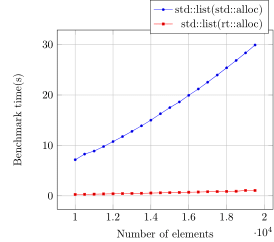
\includegraphics[scale=0.5]{fig/std_list_bench.png} }
%    \subfloat[]{ 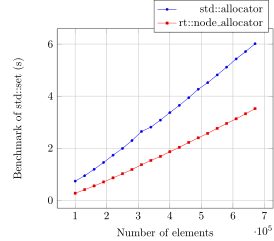
\includegraphics[scale=0.5]{fig/std_set_bench.png} }
%        \\
%    \caption[Benchmarks]
%    {Never slower than blah.}
%    \label{fig::bench}
%\end{figure}


\section{Impact on the Standard} \label{impact}

We require that all node based containers favor the overload
\texttt{allocate()} over \texttt{allocate(size\_type)}, for all node
allocations inside the container, whenever
\texttt{std::allocator\_traits} instructs them so, by means of a new
typedef
\medskip
\begin{lstlisting}
template<class Alloc>
struct allocator_traits {
  ...
  // Equal to Alloc::node_allocation_only if present,
  // std::false_type otherwise.
  using node_allocation_only = std::false_type

  // Calls a.allocate_node() if present otherwise calls
  // Alloc::allocate(1).
  pointer allocate_node(Alloc& a);

  // Calls a.deallocate_node(pointer) if present otherwise
  // calls Alloc::deallocate(p, 1).
  void deallocate_node(Alloc& a, pointer);
};
\end{lstlisting}
When \texttt{use\_node\_allocation} is not present in the allocator,
the typedef should default to \texttt{std::false\_type}.
We also propose that node-based containers should expose their node type.

The following containers are affected: \texttt{std::forward\_list},
\texttt{std::list}, \texttt{std::set}, \texttt{std::multiset},
\texttt{std::unordered\_set}, \texttt{std::unordered\_multiset},
\texttt{std::map}, \texttt{std::multimap},
\texttt{std::unordered\_map}, \texttt{std::unordered\_multimap}

\medskip
\noindent
{\bf Pure node-based}: As a result of this proposal all node based
containers mentioned above, with the exception of the unordered ones,
should support allocators that provide only the overload
\texttt{allocate()}.

\medskip
\noindent
{\bf Hybrid}: Unordered containers have to rebind twice, once
for node allocation and once for other internal data structures.
The rebound type used for node allocations should prefer the 
\texttt{allocate()} overload.

\section{Technical Specifications}

\section{Acknowledgment}

I would like thank people that give me any kind of feedback: Ville Voutilainen,
Nevin Liber, Daniel Gutson, Alisdair Meredith, David Krauss. Special thanks go
to Ion Gaztañaga for suggesting important changes in the original design and David 
Krauss for proposing a diferent approach.

\begin{thebibliography}{9}

  \bibitem{middleditch} Sean Middleditch, \url{http://www.open-std.org/jtc1/sc22/wg21/docs/papers/2015/p0038r0.html}
  \bibitem{chandler} Chandler Carruth, {\it Efficiency with Algorithms, Performance
  with Data Structures} (\url{https://www.youtube.com/watch?v=fHNmRkzxHWs})
  \bibitem{meyers} Scott Meyers, {\it Cpu Caches and Why You Care} (\url{https://www.youtube.com/watch?v=WDIkqP4JbkE})
  \bibitem{boost} \url{http://www.boost.org/doc/libs/1_58_0/boost/container/node_allocator.hpp}
  \bibitem{prop1} Ion Gazta\~ naga, \url{http://www.open-std.org/jtc1/sc22/wg21/docs/papers/2006/n2045.html}
  \bibitem{rtcpp} \url{https://github.com/mzimbres/rtcpp}
  \bibitem{alexandrescu} Andrei Alexandrescu, {\it std::allocator Is to Allocation what
  std::vector Is to Vexation} (\url{https://www.youtube.com/watch?v=LIb3L4vKZ7U})
  \bibitem{embedded} \url{http://www.open-std.org/pipermail/embedded/2014-December/000335.html}
  \bibitem{proplist} \url{https://groups.google.com/a/isocpp.org/forum/#!topic/std-proposals/ccwOpTxM_xE}

\end{thebibliography}

\appendix

\section{Alternative approaches} \label{alternative}

There are other possible approaches to support node allocation that are worth knowing
of.  I will list them here, so that the commitee can compare them.

\medskip
\noindent
{\bf Ensure \texttt{allocate(n)} is called with $n = 1$}. This seems the easiest
way to perform node allocation. Once the standard guarantees $n$ will be always $1$,
there is no more need to provide array allocation for node-based containers. The
prameter $n$ can be simply ignored. The \texttt{allocate} and\texttt{deallocate}
can be implemented in terms of node-allocation-only functions, for example
\medskip
\begin{lstlisting}
pointer allocate(std::size_t /* n is ignored */)
{
  return allocate_node();
}

void deallocate_node(pointer p, std::size_t /* n is ignored */)
{
  deallocate_node();
}
\end{lstlisting}

The problem with this approach is that it prevents array allocation inside
node-based containers which means it can be viewed as a narrowing of the
current interface.

\medskip
\noindent
{\bf Provide a \texttt{constexpr max\_size()} that returns 1}. This approach has one advantage

\begin{itemize}
\item It does not require any new member functions and typedef in the
\texttt{std::allocator\_traits}.
\end{itemize}

The disadvantages I see however are

\begin{itemize}
\item It requires the user to specialize \texttt{std::allocator\_traits} to
provide a \texttt{constexpr max\_size()} since the default is not
\texttt{constexpr}. This is not bad but I prefer to avoid it if I can.

\item Other static information like \texttt{propagate\_on\_container\_copy\_assignment}
are provided as typedef so I would prefer to keep the harmony.

\item Libraries would have to detect \texttt{constexpr}'ness and take appropriate action.
This is not much different than detecting if \texttt{node\_allocation\_only::value} is true or
false but my personal opinion is that this procedure is not elegant for standardization.

\item It sounds more like a hack of the current standard interface to achieve node
allocation than a full supported feature.

\end{itemize}


\end{document}

